% This is LLNCS.DEM the demonstration file of
% This is LLNCS.DEM the demonstration file of
% the LaTeX macro package from Springer-Verlag
% for Lecture Notes in Computer Science, version 1.1
\documentclass{llncs}
%
% Remove any % below to load the required packages
\usepackage[latin1]{inputenc}
\usepackage{amsmath}
\usepackage{listings}
\usepackage{marvosym}
\usepackage{color}
\usepackage{graphicx}
\usepackage{caption}
\usepackage{pgf}
\usepackage{tikz}
\usepackage{subfig}
\usepackage[american]{babel}
\usetikzlibrary{arrows,automata,positioning}
\usepackage{epstopdf}
\newtheorem{mydef}{Definition}
\newtheorem{mylem}{Lemma}
\usepackage{afterpage}

\renewcommand{\baselinestretch}{0.96}

\lstset{language=C,basicstyle=\small}
\lstset{numbers=left, numberstyle=\tiny, stepnumber=1, numbersep=5pt}
\lstset{tabsize=2}
\lstset{firstnumber=1}
\lstset{frame=single}
\lstset{
  language={C},
  morekeywords={enquanto,se,fim,entao,senao,retorne,faca,assume,then,end-if,end,input,output,cudaMemcpyHostToDevice,cudaMemcpyDeviceToHost,\_\_global\_\_}
}
\hyphenation{port-a-ble}

\newcommand{\comment}[1]{}

\begin{document}

\title{ESBMC-GPU}
\subtitle{A Context-Bounded Model Checking Tool \\ to Verify CUDA Programs}
%\author{Felipe~R.~Monteiro$^{1}$, Isabela~S.~Silva$^{1}$,\\Lucas~C.~Cordeiro$^{1,2}$, and Eddie~B.~de~Lima~Filho$^{1,3}$}

%\institute{$^{1}$Federal University of Amazonas, Brazil \\ 
%$^{2}$University of Oxford, United Kingdom \\
%$^{3}$ FPF Tech, Brazil}% \\

%
%\date{Received: date / Revised version: date}
% The correct dates will be entered by Springer
%

%\authorrunning{F.~R.~Monteiro et al.}
\titlerunning{ESBMC-GPU: A Context-Bounded Model Checking Tool to Verify CUDA Programs}

\maketitle

\begin{abstract}
The Compute Unified Device Architecture (CUDA) is a programming model used for exploring the advantages of Graphics Processing Unit (GPU) devices, through parallelization and specialized functions and features. However, as in other development platforms, errors may occur, due to traditional software creation processes, which may even compromise the execution of an entire system. In order to address such a problem, ESBMC-GPU was developed, as an extension to the Efficient SMT-Based Context-Bounded Model Checker (ESBMC). In summary, ESBMC processes input code through ESBMC-GPU and an abstract representation of the standard CUDA libraries, with the goal of checking a set of desired properties. Experimental results showed that ESBMC-GPU was able to correctly verify $82$\% of the chosen benchmarks and also overcame other existing GPU verifiers.%, mainly due to their inability in detecting array out-of-bounds and data race violations.
\end{abstract}

%\keywords{GPU verification; formal methods; model checking; CUDA.}

%=-=-=-=-=-=-=-=-=-=-=-=-=-=-=-=-=-=-=-=-=-=-=-=-=-=-=
\section{Introduction} 
\label{sec:intro}
%=-=-=-=-=-=-=-=-=-=-=-=-=-=-=-=-=-=-=-=-=-=-=-=-=-=-=

The Compute Unified Device Architecture (CUDA) is a development framework that makes use of the architecture and processing power of Graphics Processing Units (GPUs)~\cite{cuda:2012}. Indeed, CUDA is also an Application Programming Interface (API), through which a GPU's parallelization scheme and tools can be accessed, with the goal of executing kernels. However, source code is still written by human programmers, which may result in arithmetic overflow, division by zero, and other violation types. In addition, given that CUDA allows parallelization, problems related to the latter can be identified, due to thread scheduling~\cite{betts:2012}.

In order to address that problem, an extension to the Efficient SMT-Based Context-Bounded Model Checker (ESBMC)~\cite{cordeiro:2012} was developed, named as ESBMC-GPU~\cite{Pereira15,Pereira16,pereira:2016}, with the goal of verifying CUDA-based programs (available online at \texttt{www.esbmc-gpu.org}). ESBMC-GPU consists of an extension for parsing CUDA source code ({\it i.e.}, a front-end to ESBMC) and a CUDA operational model (COM), which is an abstract representation of the standard CUDA libraries ({\it i.e.}, the native API) that conservatively approximates their semantics. 

A distinct difference of ESBMC-GPU, when compared with other approaches \cite{betts:2012,Li:2010,Li:2012,civl:2015}, is the use of Bounded Model Checking (BMC) allied to Satisfiability Modulo Theories (SMT), with explicit state-space exploration~\cite{cordeiro:2012}. Concurrency problems are tackled, up to an unwinding bound, while each interleaving itself is symbolically handled. However, even with BMC, space-state exploration may become a very time-consuming task, which is alleviated through state hashing and Monotonic Partial Order Reduction (MPOR)~\cite{KahlonWG09}. As a consequence, redundant interleavings are eliminated, without ignoring a program's behavior.


Finally, existing GPU verifiers normally ignore some aspects related to memory leak, data transfer, and overflow, which are normally present in CUDA programs. The proposed approach, in turn, explicitly addresses them, through an accurate checking procedure, which even considers data exchange between main program and kernel. Of course, that results in higher verification times, but more errors can then be identified and later corrected, in another development cycle.

%=-=-=-=-=-=-=-=-=-=-=-=-=-=-=-=-=-=-=-=-=-=-=-=-=-=-=
%\subsection{Existing GPU Verifiers}
%\label{sec:related-work}
%=-=-=-=-=-=-=-=-=-=-=-=-=-=-=-=-=-=-=-=-=-=-=-=-=-=-=

\textbf{Existing GPU Verifiers}. GPUVerify~\cite{betts:2012} is based on Synchronous Delayed Visibility, which focus on detecting data race and barrier divergence, while reducing kernel verification procedures to the analysis of sequential programs. Symbolic Executor with Static Analysis (SESA)~\cite{sesa:2014} and GPU + KLEE (GKLEE)~\cite{Li:2012} are concrete plus symbolic (\textit{concolic}) execution tools. Initially, GKLEE modeled every original thread, which was later improved by taking into account symmetry, and it considers both kernel and main function, while checking barrier synchronization and data race, among others. SESA combines equivalent flows, which results in great performance improvement, focus on data race detection, and does not verify the main function. Prover of User GPU Programs (PUG)~\cite{Li:2010} is based on SMT solvers and applies symbolic static analysis to each kernel, but requires user annotations. CIVL~\cite{civl:2015} generates an abstract syntax tree and supports analysis and transformations. Besides, it also verifies concurrent programs with partial order reduction, which makes it very similar to the solution proposed here. Given that its support to CUDA libraries is still under development, CIVL is an interesting approach for checking simple CUDA programs.

%=-=-=-=-=-=-=-=-=-=-=-=-=-=-=-=-=-=-=-=-=-=-=-=-=-=-=
\section{Architecture and Implementation}
\label{sec:arch}
%=-=-=-=-=-=-=-=-=-=-=-=-=-=-=-=-=-=-=-=-=-=-=-=-=-=-=

ESBMC-GPU builds on ESBMC, which is an open source context-bounded model checker based on SMT solvers~\cite{cordeiro:2012} for ANSI-C/C$++$ programs. ESBMC-GPU adds four essential models to ESBMC, as described below.\\

\noindent \textbf{CUDA Operational Model.} An operational model for CUDA libraries, in conjunction with ESBMC, provides support to CUDA functionalities, as shown in Fig.~\ref{figure:arch}. Such an approach, which was previously attempted in the verification of C++ programs~\cite{ramalho:2013,garcia:2016}, consists in an abstract representation that reliably approximates the CUDA library's semantics. However, COM incorporates pre- and post-conditions as assertions into verification processes, as shown in Fig.~\ref{figure:om}, which enables ESBMC-GPU to verify specific properties (cf. Sec.~\ref{sec:features}). Indeed, COM allows the necessary control for performing code analysis, where both CUDA operation and knowledge for model checking its properties are available.

\begin{figure}[htb]
  \centering
  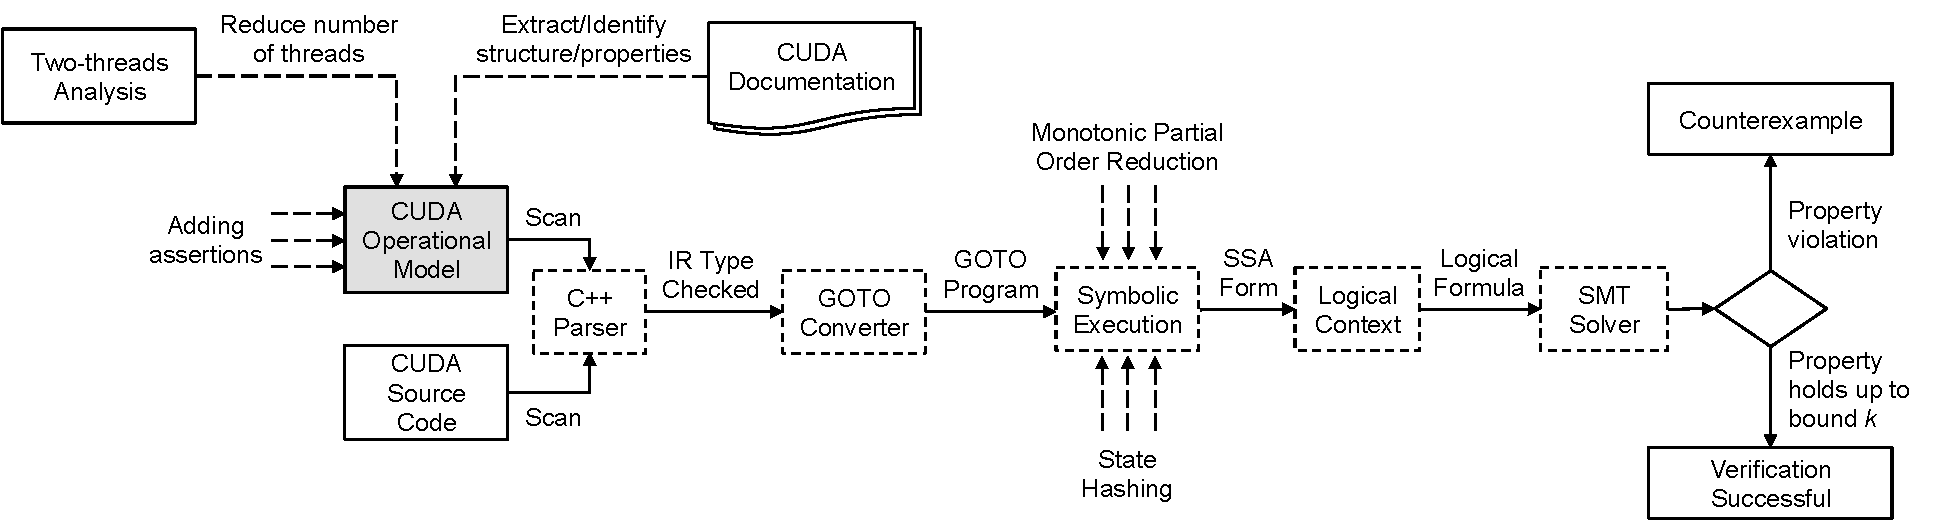
\includegraphics[width=5in]{figures/arch.pdf}
  \caption{Overview of ESBMC-GPU's architecture.}
  %\caption{Connecting the operational model for CUDA library to ESBMC architecture.}
  \label{figure:arch}
\end{figure}



ESBMC was designed to handle multi-threaded software, through the use of the Portable Operating System Interface (POSIX -- ISO/IEC 9945).
%~\cite{posix:2008}
Thus, ESBMC-GPU applies a combination between processing methods used by Central Processing Units (CPUs) and the POSIX library, where thread instructions can interleave to create execution paths. Particularly, COM simulates the behavior of kernel calls using pthread functions ({\it e.g.}, {\tt pthread\_create}) and combines that with ESBMC, in order to check data race and specific C/C++ programming language failures ({\it e.g.}, array out-of-bounds and pointer safety).\\
%Additionally, ESBMC-GPU employs symbolic state hashing~\cite{Morse11}, monotonic partial order reduction (MPOR)~\cite{morse:2015}, and the two-thread analysis~\cite{pereira:2016}, in order to prune the state space exploration.

\begin{figure}[htb]
  \centering
  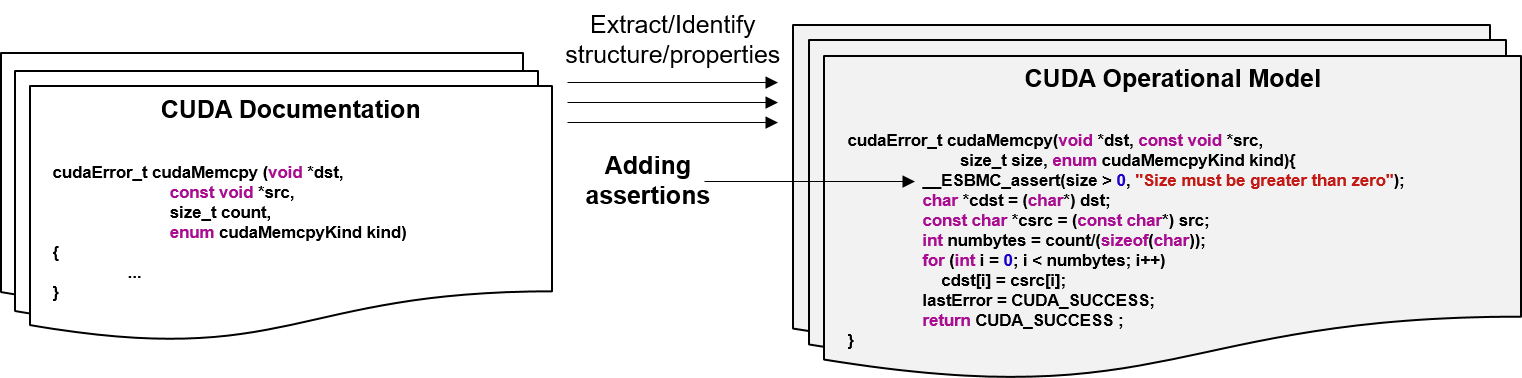
\includegraphics[width=4.5in]{figures/cuda-om.png}
  \caption{CUDA operational model development process.}
  \label{figure:om}
\end{figure}


\noindent \textbf{Two-threads Analysis.} Similarly to GPUVerify~\cite{betts:2012} and PUG~\cite{Li:2010}, ESBMC-GPU also reduces the number of threads, during the verification of CUDA programs, to two, considering a NVIDIA Fermi GPU architecture, in order to improve verification time and avoid the state-space explosion problem. In CUDA programs, whilst threads execute the same parametrized kernel, only two threads are necessary for conflict check. Thus, such an analysis ensures that errors ({\it e.g.}, data races) detected between two threads, in a given subgroup and due to unsynchronized accesses to shared variables, are enough to justify a property violation.\\

\noindent \textbf{State Hashing.} ESBMC-GPU applies state hashing to further eliminate redundant interleavings and reduce state space, based on SHA256 hashes.\\%, due to the low the likelihood regarding collisions. \\
%~\cite{FIPS:2002}

\noindent \textbf{Monotonic Partial Order Reduction.} MPOR is used to reduce the number of thread interleavings, by classifying transitions inside a program as dependent or independent. As a consequence, it is possible to determine whether interleaving pairs always lead to the same state and then remove duplicates in a reachability tree, without ignoring any aspect of a program's behavior.

%In addition to both techniques, 

%=-=-=-=-=-=-=-=-=-=-=-=-=-=-=-=-=-=-=-=-=-=-=-=-=-=-=
\section{Functionalities}
\label{sec:features}
%=-=-=-=-=-=-=-=-=-=-=-=-=-=-=-=-=-=-=-=-=-=-=-=-=-=-=

Through the integration of COM into ESBMC, ESBMC-GPU is able to analyze CUDA programs and verify the following properties:

\begin{itemize}
	\item \textbf{Data race.\ } ESBMC-GPU checks data race conditions, in order to detect if multiple threads perform unsynchronized access to shared-memory locations.
	
	\item \textbf{Pointer safety. } ESBMC-GPU also ensures that {\it (i)} a pointer offset does not exceed object bounds and {\it (ii)} a pointer is neither {\tt NULL} nor invalid.
	
	\item \textbf{Array bounds.\ } ESBMC-GPU performs array-bound checking, in order to ensure that any variable, used as an array index, is within known bounds.
	
	\item \textbf{Arithmetic under- and overflow.\ } ESBMC-GPU checks whether a sum or product exceeds the memory limits that a variable can handle.%, which can cause an error capable of spreading through the entire execution path.
	
	\item \textbf{Division by zero.\ } ESBMC-GPU analyzes whether denominators, in arithmetic expressions, lead to a division by zero.
	
	\item \textbf{User-specified assertions.\ } ESBMC-GPU considers all assertions specified by users, which is essential to a thorough verification process.%, as some specific possible violations must be explicitly pointed out.
\end{itemize}

%=-=-=-=-=-=-=-=-=-=-=-=-=-=-=-=-=-=-=-=-=-=-=-=-=-=-=
\section{Usage Aspects}
\label{subsec:usage}
%=-=-=-=-=-=-=-=-=-=-=-=-=-=-=-=-=-=-=-=-=-=-=-=-=-=-=

In order to verify CUDA code, users must slightly modify one specific parameter, in a given program. In particular, the call %``{\tt kernel<<< blocks, threads >>>(kernel-parameters)}'' must be changed to ``{\tt ESBMC\_verify\_kernel(<kernel>, <blocks>, <threads>, <kernel-parameters>)}'', where {\tt <kernel>} is the kernel to be verified, {\tt <blocks>} is the number of blocks, {\tt <threads>} is the number of threads, and {\tt <kernel-parameters>} is the kernel function's parameters. After the required amendments, users must call ``\texttt{esbmc-gpu} \emph{\tt <file>.cu} {\tt --unwind <$k$>}  {\tt --context-switch <$c$>}  {\tt --state-hashing} {\tt -I <path-to-CUDA-OM>}'', where {\tt $<$file$>$.cu} is the CUDA program to be verified, {\tt <$k$>} is the maximum loop unrolling, {\tt <$c$>} is a context-switch bound among all threads, {\tt --state-hashing} reduces redundant interleavings, and {\tt $<$path-to-CUDA-OM$>$} is the location of the COM library. In addition, the flag {\tt --data-races-check} must be added at the end of the aforementioned command line, in order to check data races.

\begin{center}
\vspace{1 mm}
{\tt kernel<<< blocks, threads >>>(kernel-parameters)}
\vspace{1 mm}
\end{center}

\noindent must be transformed to the following ESBMC-GPU intrinsic function: called {\tt ESBMC\_verify\_kernel()}, which takes as arguments: the kernel to be verified, the number of blocks, the number of threads, and the kernel parameters, respectively.

\begin{center}
\vspace{1 mm}
\noindent {\tt ESBMC\_verify\_kernel(<kernel>, <blocks>,}

\noindent {\tt <threads>, <kernel-parameters>)},
\vspace{1 mm}
\end{center}

\noindent where {\tt <kernel>} is the kernel to be verified, {\tt <blocks>} is the number of blocks, {\tt <threads>} is the number of threads, and {\tt <kernel-parameters>} is the kernel function's parameters. After the required amendments, the user must call the ESBMC-GPU v$2.0$ command-line version, using

\begin{center}
\vspace{1 mm}
\noindent \texttt{esbmc-gpu} \emph{\tt <file>.cu} {\tt --unwind <$k$>}  {\tt --context-switch <$c$>} % --force-malloc-success}

\noindent {\tt --state-hashing} {\tt -I <path-to-CUDA-OM>},
\vspace{1 mm}
\end{center}

where {\tt $<$file$>$.cu} is the CUDA program to be verified, {\tt <$k$>} is the maximum loop unrolling, {\tt <$c$>} is a context-switch bound among all threads, {\tt --state-hashing} reduces redundant interleavings, and {\tt $<$path-to-CUDA-OM$>$} is the location of the COM library. In addition, the flag {\tt --data-races-check} must be added at the end of the aforementioned command line, in order to check data races.

In summary, if no bug is found, up to a $k$-depth unwinding and a $c$ context-bound, ESBMC-GPU reports {\tt VERIFICATION SUCCESSFUL}. Conversely, it reports {\tt VERIFICATION FAILED}, along with a counterexample, which contains all necessary information for identifying and reproducing the respective error. It is worth mentioning that counterexamples are not only recipients that contain the necessary information for reaching an error state, but it can also be used for implementing proper code correction, even automatically.

%=-=-=-=-=-=-=-=-=-=-=-=-=-=-=-=-=-=-=-=-=-=-=-=-=-=-=
\section{Experimental Evaluation}
\label{sec:effectiveness}
%=-=-=-=-=-=-=-=-=-=-=-=-=-=-=-=-=-=-=-=-=-=-=-=-=-=-=

%In order to evaluate ESBMC-GPU's precision and performance, we have developed an automated test suite, which covers all basic functions that are commonly used by real CUDA-based applications. 
The chosen benchmark suite comprises $20$ CUDA kernels from NVIDIA GPU Computing SDK v$2$.$0$, $20$ CUDA kernels from Microsoft C$++$ AMP Sample Projects%~\cite{microsoft:2012}
, and $104$ CUDA-based programs that explore a wide range of CUDA functionalities~\cite{cuda:2012}. In summary, the chosen suite contains $47.4$\% bug-free and $52.6$\% buggy benchmarks, which tackle data race, arithmetic operations, pointer assignment, {\tt \_\_device\_\_} function calls, general ANSI-C functions ({\it e.g.}, \texttt{memset}), general CUDA functions ({\it e.g.}, \texttt{cudaMemcpy}), general libraries in CUDA ({\it e.g.}, \texttt{curand.h}), and the ability to work with variables, type modifiers ({\it e.g.}, \texttt{unsigned}), pointers, type definitions, and intrinsic CUDA variables ({\it e.g.}, \texttt{uint4}).  The present experiments answer two research questions:

%\textcolor{blue}{existe outra informacao sobre a test suite que seria interessante mencionar? falta eu colocar a porcentagem de testes com e sem erro, mas para isso preciso conversar com os membros da equipe}

%\textcolor{red}{seria possivel explicar mais a escolha dos benchmarks? quantos utilizam funcionalidades especificas cuda? quantos permitem avaliar data-race? quantos errados e quantos sem erros?} 

\begin{enumerate}

%\item {\bf (sanity check)} Which results does ESBMC-GPU obtain upon verifying benchmarks from the automated test suite?
\item How accurate is ESBMC-GPU when verifying the chosen test suite?

%\textcolor{red}{na verdade, nao deveriamos responder o quao correto o nosso eh e nao apenas se ele eh melhor ou pior?}

%\item {\bf (compare software performance)} What is ESBMC-GPU performance when compared to GKLEE, GPUVerify, PUG, and CIVL?
\item How does ESBMC-GPU compare to other existing verifiers?

%\textcolor{red}{na verdade, uma pergunta seria: o quao ``adequado'' o noss eh? ele jah analisa coisas que os outros ignoram... seria bom colocar isso aqui pois ateh deixaria diferente do artigo}

\end{enumerate}

\noindent In order to answer both questions, all benchmarks were verified with $5$ GPU verifiers (ESBMC-GPU, GKLEE, GPUVerify, PUG, and CIVL), on an otherwise idle Intel Core i$7$-$4790$ CPU $3$.$60$ GHz, with $16$ GB of RAM and a Linux OS. All times were measured by the UNIX time command, in seconds. An overview of the experimental results is shown in Fig.~\ref{figure:experimental}, where {\it True} represents bug-free benchmarks, {\it False} represents buggy benchmarks, {\it Not supported} represents benchmarks that could not be verified, {\it Correct} represents the percentage of benchmarks correctly verified, and {\it Incorrect} represents the percentage of benchmarks incorrectly verified. As one may notice, the present experimental results show that ESBMC-GPU reached a successful verification rate of approximately $82\%$, while GKLEE, GPUVerify, PUG, and CIVL reported $70\%$, $57\%$, $35\%$, and $31\%$, respectively. More precisely, ESBMC-GPU support the verification of benchmarks related to array bounds ($3$\%), assertive statements ($5$\%), data race ($11$\%), {\tt NULL} pointers ($3$\%), and other specific CUDA functionalities ($60$\%).

{\bf Limitations.} ESBMC-GPU was unable to correctly verify $27$ benchmarks, which are related to constant memory access ($2$\%), the use of CUDA's specific libraries ($4.5$\%), and the use of pointers to functions, structures, and {\tt char} type variables, when used as kernel call arguments ($8.5$\%). In addition, ESBMC-GPU only reported $1$\% of false positive and $2$\% false negative results.

%\textcolor{red}{aqui ficou meio largado... o nosso eh bom para caralho e isso tem que ficar muito claro... comente mais as duas porcentagens que totalizam os 82\%, no ESBMC-GPU... e qual foi realmente o acerto... dos erros existentes, quantos acertamos?} \textcolor{blue}{Preciso da informacao de quantos estao com bugs, como mencionado acima...}
%In addition, ESBMC-GPU had $23$ benchmarks that were not supported. These are related to constant memory access ($3$), the use of CUDA's specific libraries (\textit{e.g., curand.h}) ($7$), and the use of pointers to functions, structures, and char type variables used as kernel call arguments ($13$). 

{\bf Performance.} MPOR resulted in a performance improvement of approximately $80\%$, by decreasing the verification time from $16$ to $3$ hours, while the two-threads analysis further reduced that to $811$ seconds. Although such techniques have considerably improved the ESBMC-GPU's performance, it still takes longer than the other evaluated tools:  GKLEE ($128$ sec), GPUVerify ($147$ sec), PUG ($12$ sec), and CIVL ($158$ sec). This is due to thread interleavings, which combine symbolic model checking with explicit state-space exploration. In addition, even though ESBMC-GPU reports the highest verification time, it still presents the highest accuracy, with less than $6$ seconds per benchmark.%, which shows that it is a feasible tool regarding the verification of CUDA-based applications. 

%\textcolor{red}{tudo bem... mas como melhorar? tem que mencionar que se tempo nao for um problema, isso eh completamente aceitavel... principalmente se for tudo automatico... o desenvolvedor vai deixar lah rolando, almoca e depois volta... entendeu?}

%\textcolor{red}{alem disso, eh bom mencionar quem eh mais adequado a umd ado tipo de erros... ganhamos em tudo ou um dos outros eh melhor em uma dada condicao?... seria bom separar erros por categoria}

\begin{figure}[htb]
  \centering
  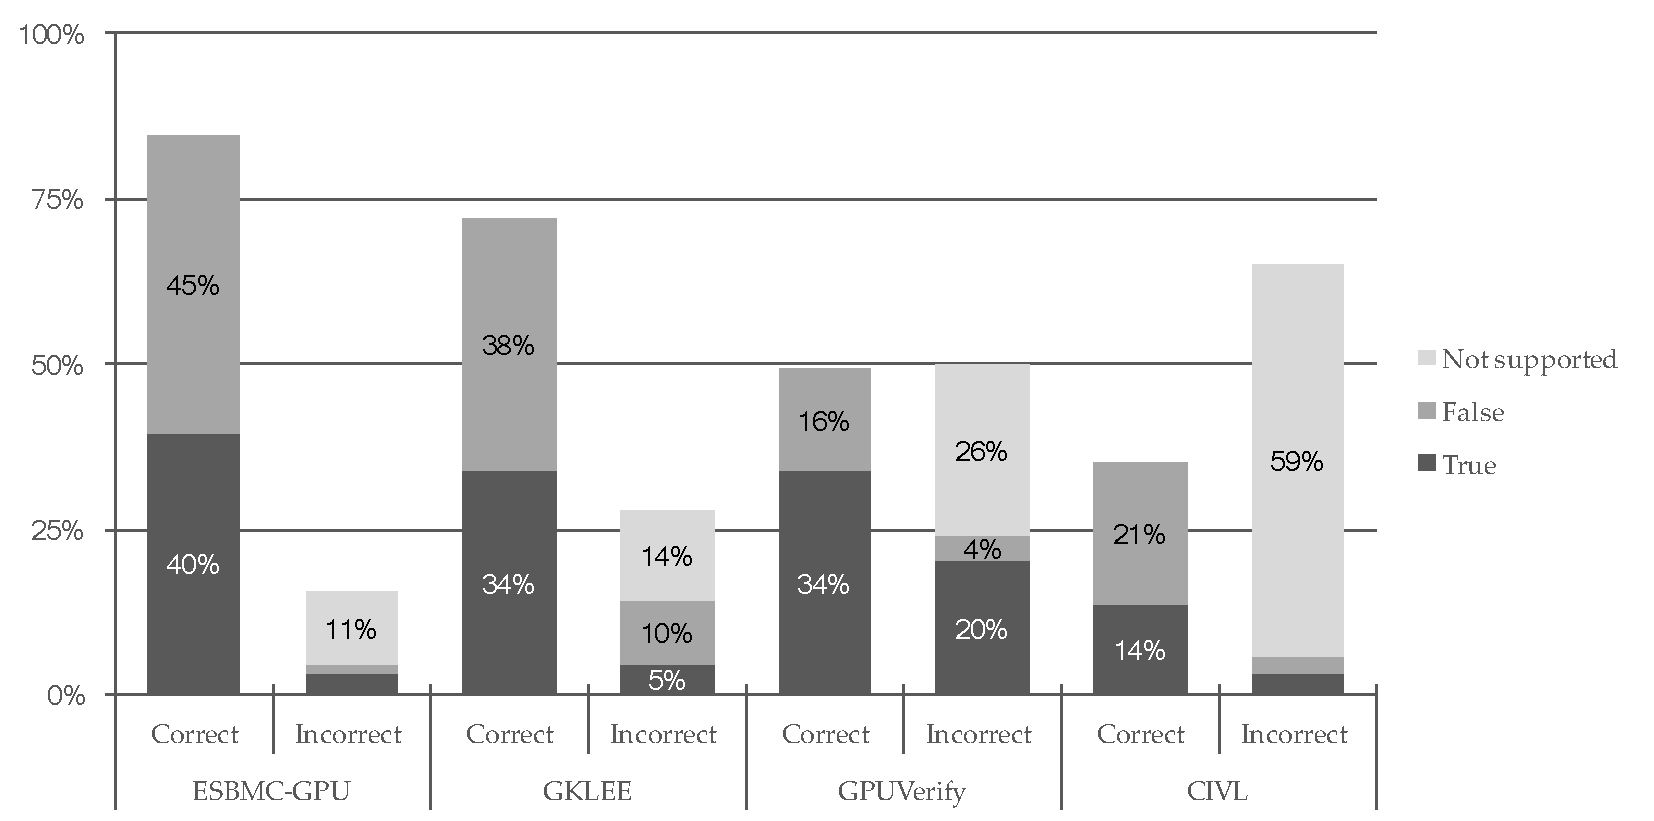
\includegraphics[width=5in]{figures/experimental-results.pdf}
  \caption{Experimental evaluation of ESBMC-GPU against other verifiers.}
  \label{figure:experimental}
\end{figure}

\noindent \textbf{Availability of Data and Tools.} The performed experiments are based on a set of publicly available benchmarks. All benchmarks, tools, and results, associated with the current evaluation, are available on {\tt http://esbmc-gpu.org/}.

%=-=-=-=-=-=-=-=-=-=-=-=-=-=-=-=-=-=-=-=-=-=-=-=-=-=-=
\section{Conclusions and Future Work}
\label{sec:conc}
%=-=-=-=-=-=-=-=-=-=-=-=-=-=-=-=-=-=-=-=-=-=-=-=-=-=-=

ESBMC-GPU is an SMT-based BMC tool that recognizes CUDA directives, further simplifies verification models, and provides fewer incorrect results, if compared with GKLEE, GPUVerify, PUG, and CIVL. In addition, it presents an improved ability to detect array out-of-bounds and data race violations. Future work aims to support stream interleaving and implement further techniques to reduce the number of thread interleavings by taking into account the GPU symmetry.

%\textcolor{red}{aqui eh bom mencionar numeros... quanto eh melhor? apenas resuma o que jah tem acima... e para melhorar a velocidade?}

%\noindent \textbf{Acknowledgements.} This paper is based on research sponsored by the Institute of Development and Technology (INdT) and by the National Council for Scientific and Technological Development (CNPq) under agreement number $475647/2013-0$.

\begin{thebibliography}{25}

\bibitem{cuda:2012}
Cheng, J., Grossman, M., and McKercher, T.
\newblock {\em {Professional CUDA C Programming}}.
\newblock {John Wiley and Sons, Inc.} 2014.

%\bibitem{gpu:2010}
%Kirk, D. and Hwu, W.
%\newblock {\em {Programming Massively Parallel Processors}}.
%\newblock Elsevier, 2010.

\bibitem{betts:2012}
Betts, A., Chong, N., Donaldson, A., Qadeer, S., and Thomson, P.
\newblock {\em{GPUVerify: A Verifier for {GPU} Kernels}}.
\newblock {OOPSLA} 2012; 113--132.

\bibitem{cordeiro:2012}
Cordeiro, L. and {\it et al.} %, Fischer, B., and Marques{-}Silva, J.
\newblock {\em{SMT-Based Bounded Model Checking for Embedded {ANSI-C} Software}}.
\newblock {IEEE} Trans. Software Eng. 2012; 38(4):957--974.

\bibitem{Pereira15}
Pereira, P., Albuquerque, H., Marques, H., Silva, I., Carvalho, C., Santos, V., Ferreira, R., and Cordeiro, L.
\newblock {\em{Verifica\c{c}\~ao de Kernels em Programas CUDA usando Bounded Model Checking.}} 
\newblock {WSCAD-SSC} 2015; 24--35.

\bibitem{Pereira16}
Pereira, P., Albuquerque, H., Marques, H., Silva, I., Carvalho, C., Santos, V., Ferreira, R., and Cordeiro, L.
\newblock {\em{Verifying CUDA Programs using SMT-Based Context-Bounded Model Checking.}} 
\newblock {SAC SVT track 2016; 1648--1653.}

\bibitem{pereira:2016}
Pereira, P., Albuquerque, H., Silva, I., Marques, H., Monteiro, F., Ferreira, R., and Cordeiro, L.
\newblock {\em{SMT-Based Context-Bounded Model Checking for CUDA Programs}}.
\newblock Concurrency Computat.: Pract. Exper. 2016; ({\it to appear}).

\bibitem{Li:2010}
Li, G. and Gopalakrishnan, G.
\newblock {\em{Scalable SMT-based Verification of GPU Kernel Functions}}.
\newblock {FSE} 2010; 187--196.

\bibitem{Li:2012}
Li, G., Li, P., Sawaya, G., Gopalakrishnan, G., Ghosh, I., and Rajan, S.
\newblock {\em{GKLEE: Concolic Verification and Test Generation for GPUs.}}
\newblock {PPoPP} 2012; 215--224.

\bibitem{civl:2015}
Zheng, M., Rogers, M., Luo, Z., Dwyer, M., and Siegel, S.
\newblock {\em{{CIVL}: Formal Verification of Parallel Programs}}.
\newblock {ASE} 2015; 830--835.

\bibitem{KahlonWG09}
Kahlon V, Wang C, Gupta A.
\newblock {\em{Monotonic Partial Order Reduction: An Optimal Symbolic Partial Order
  Reduction Technique}}.
\newblock {CAV} 2009; 398--413.

\bibitem{sesa:2014}
Li, P., Li, G., and Gopalakrishnan, G.
\newblock {\em{Practical Symbolic Race Checking of {GPU} Programs}}.
\newblock {SC} 2014; 179--190.

%\bibitem{Biere:2009}
%Biere, A.
%\newblock {\em{Bounded Model Checking. Handbook of Satisfiability}}. 
%\newblock {IOS Press} 2009; 457--481.

%\bibitem{Barrett:2009}
%Barrett C, Sebastiani R, Seshia S, Tinelli C.
%\newblock {\em{ Satisfiability Modulo Theories. Handbook of Satisfiability}}.
%\newblock {IOS Press} 2009; 825--885.

%\bibitem{cordeiro:2011}
%Cordeiro, L. and Fischer, B.
%\newblock {\em{Verifying Multi-threaded Software using SMT-based Context-Bounded
%  Model Checking}}.
%\newblock {ICSE} 2011; 331--340.

%\bibitem{KahlonWG09}
%Kahlon V, Wang C, Gupta A.
%\newblock {\em{Monotonic Partial Order Reduction: An Optimal Symbolic Partial Order
%  Reduction Technique}}.
%\newblock {CAV} 2009; 398--413.

%\bibitem{Morse11}
%Morse, J., Cordeiro, L., Nicole, D., and Fischer, B.
%\newblock {\em{Context-Bounded Model Checking of LTL Properties for ANSI-C Software.}} 
%\newblock {SEFM} 2011; 302--317.

%\bibitem{Morse:15}
%Morse, J. and {\it et al.} %, Cordeiro, L., Nicole, D., and Fischer, B.
%\newblock {\em{Model checking LTL properties over ANSI-C programs with bounded traces.}} 
%\newblock {Software and System Modeling} 2015; 14(1): 65--81.

\bibitem{ramalho:2013}
Ramalho, M., Freitas, M., Sousa, F., Marques, H., Cordeiro, L., and Fischer, B.
\newblock {\em{SMT-Based Bounded Model Checking of C++ Programs}}.
\newblock {{ECBS}} 2013; 147--156.

%\bibitem{monteiro:2015}
%Monteiro, F., Cordeiro, L., de Lima Filho, E. 
%\newblock {\em {Bounded Model Checking of C++ Programs Based on the Qt Framework}}. 
%\newblock {GCCE} 2015; 179--447.
%\newblock {DOI=http://dx.doi.org/10.1109/GCCE.2015.7398699}}

\bibitem{garcia:2016}
Garcia, M., Monteiro, F., Cordeiro, L., de Lima Filho, E. 
\newblock {\em {ESBMC$^{QtOM}$: A Bounded Model Checking Tool to Verify Qt Applications}}. 
\newblock {SPIN} 2016; 97--103.
%\newblock {DOI=http://dx.doi.org/10.1007/978-3-319-32582-8\_6}}

%\bibitem{posix:2008}
%Institute of Electrical and Electronics Engineers, Inc.
%\newblock {\em {IEEE Standard for Information Technology - Portable Operating System Interface (POSIX) Base Specifications, IEEE Std 1003.1-2008 (Revision of IEEE Std 1003.1-2004)}}.
%\newblock {IEEE} 2008.

%\bibitem{morse:2015}
%Morse, J.
%\newblock {\em {Expressive and Efficient Bounded Model Checking of Concurrent Software}}.
%\newblock {University of Southampton, PhD Thesis} 2015.

%\bibitem{cudaproguide:2015}
%NVIDIA.
%\newblock {\em {CUDA C Programming Guide}}.
%\newblock NVIDIA Corporation 2015.

%\bibitem{toolkit:2015}
%NVIDIA.
%\newblock {\em {CUDA Toolkit Release Archive}}. 
%\newblock \url{https://developer.nvidia.com/cuda-toolkit-archive}, 2015.

%\bibitem{microsoft:2012}
%Microsoft Corporation.
%\newblock {\em {C++ AMP sample projects for download (MSDN blog)}}. 
%\newblock \url{blogs.msdn.com/b/nativeconcurrency/archive/2012/01/30/c-amp-sample-projects-for-download.aspx}, 2012.

%\bibitem{FIPS:2002}
%Federal Information Processing Standard 180-2. 
%\newblock {\em {Secure Hash Standard.}}
%\newblock National Institute of Standards and Technology, 2002.

\end{thebibliography}

\newpage

%%%%%%%%%%%%%%%%%%%%%%%%%%%%%%%%%%%%
\section*{Appendix}
%%%%%%%%%%%%%%%%%%%%%%%%%%%%%%%%%%%%

\noindent The presentation plan of our work consists mainly of three parts. First, a brief motivation about general bugs in CUDA-based programs and how our present approach can assist CUDA developers to detect those bugs. Second, an overview about the ESBMC-GPU implementation and its verification approach. Third, a quick demonstration of ESBMC-GPU command-line version, using CUDA kernels from the developed benchmark test suite.
\\
\begin{enumerate}
  \item Introduction and Motivation (20\%)
  \\
  \begin{itemize} 
     \item Brief introduction about CUDA, from the perspective of a parallel computing platform and API model:
        \begin{itemize}
		\item Present the motivation as described by NVIDIA to configure GPUs;
		\item Show initial applications in graphical processing in games applications (especially those that require high computational power);
		\item Demonstrate further applications to biomedicine, air traffic control, and weather simulation. \\
	\end{itemize}
	
     \item Typical Programming Errors in CUDA:
         \begin{itemize}
		\item Show that arithmetic under- and overflow, buffer overflow, pointer safety, and division by zero are also common source of errors in CUDA programs;
		\item Emphasize that data race conditions, shared memory, and barrier divergence play an important role in CUDA-based program verification.
			\begin{enumerate}
				\item Demonstrate that all those errors lead to incorrect results during the program execution; and
				\item They are hard to detect due to the parallel operations. \\
			\end{enumerate}
	\end{itemize}
	
     \item Ensure code correctness in (critical) GPU-based applications.
         \begin{itemize}
		\item Exploit SMT-based context-BMC to verify CUDA-based programs.
			\begin{enumerate}
				\item Present an operational model for the CUDA platform, which consists of pre- and post-conditions and simulation features;
				\item Apply SMT-based context-bounded model checking to CUDA-based programs using MPOR, state-hashing, and two-thread analysis;
				\item Show the experimental results of ESBMC-GPU if compared to other state-of-art software verifiers for CUDA programs.\\
			\end{enumerate}
	\end{itemize}
	
  \end{itemize}
 
  \item ESBMC-GPU Implementation Aspects (20\%)\\
  \begin{itemize}
     \item Describe all properties that are currently supported by the ESBMC-GPU tool, which are:
     	\begin{itemize}
		\item Data race;
		\item Pointer safety (enabled by default);
		\item Memory leaks;
		\item Array bounds (enabled by default);
		\item Arithmetic under- and overflow;
		\item Division by zero (enabled by default);
		\item User-specified assertions.\\
	\end{itemize}

     \item ESBMC-GPU implementation and architecture:
      \begin{itemize}
      	\item CUDA Operational model;
	
		\begin{figure}[htb]
  			\centering
  			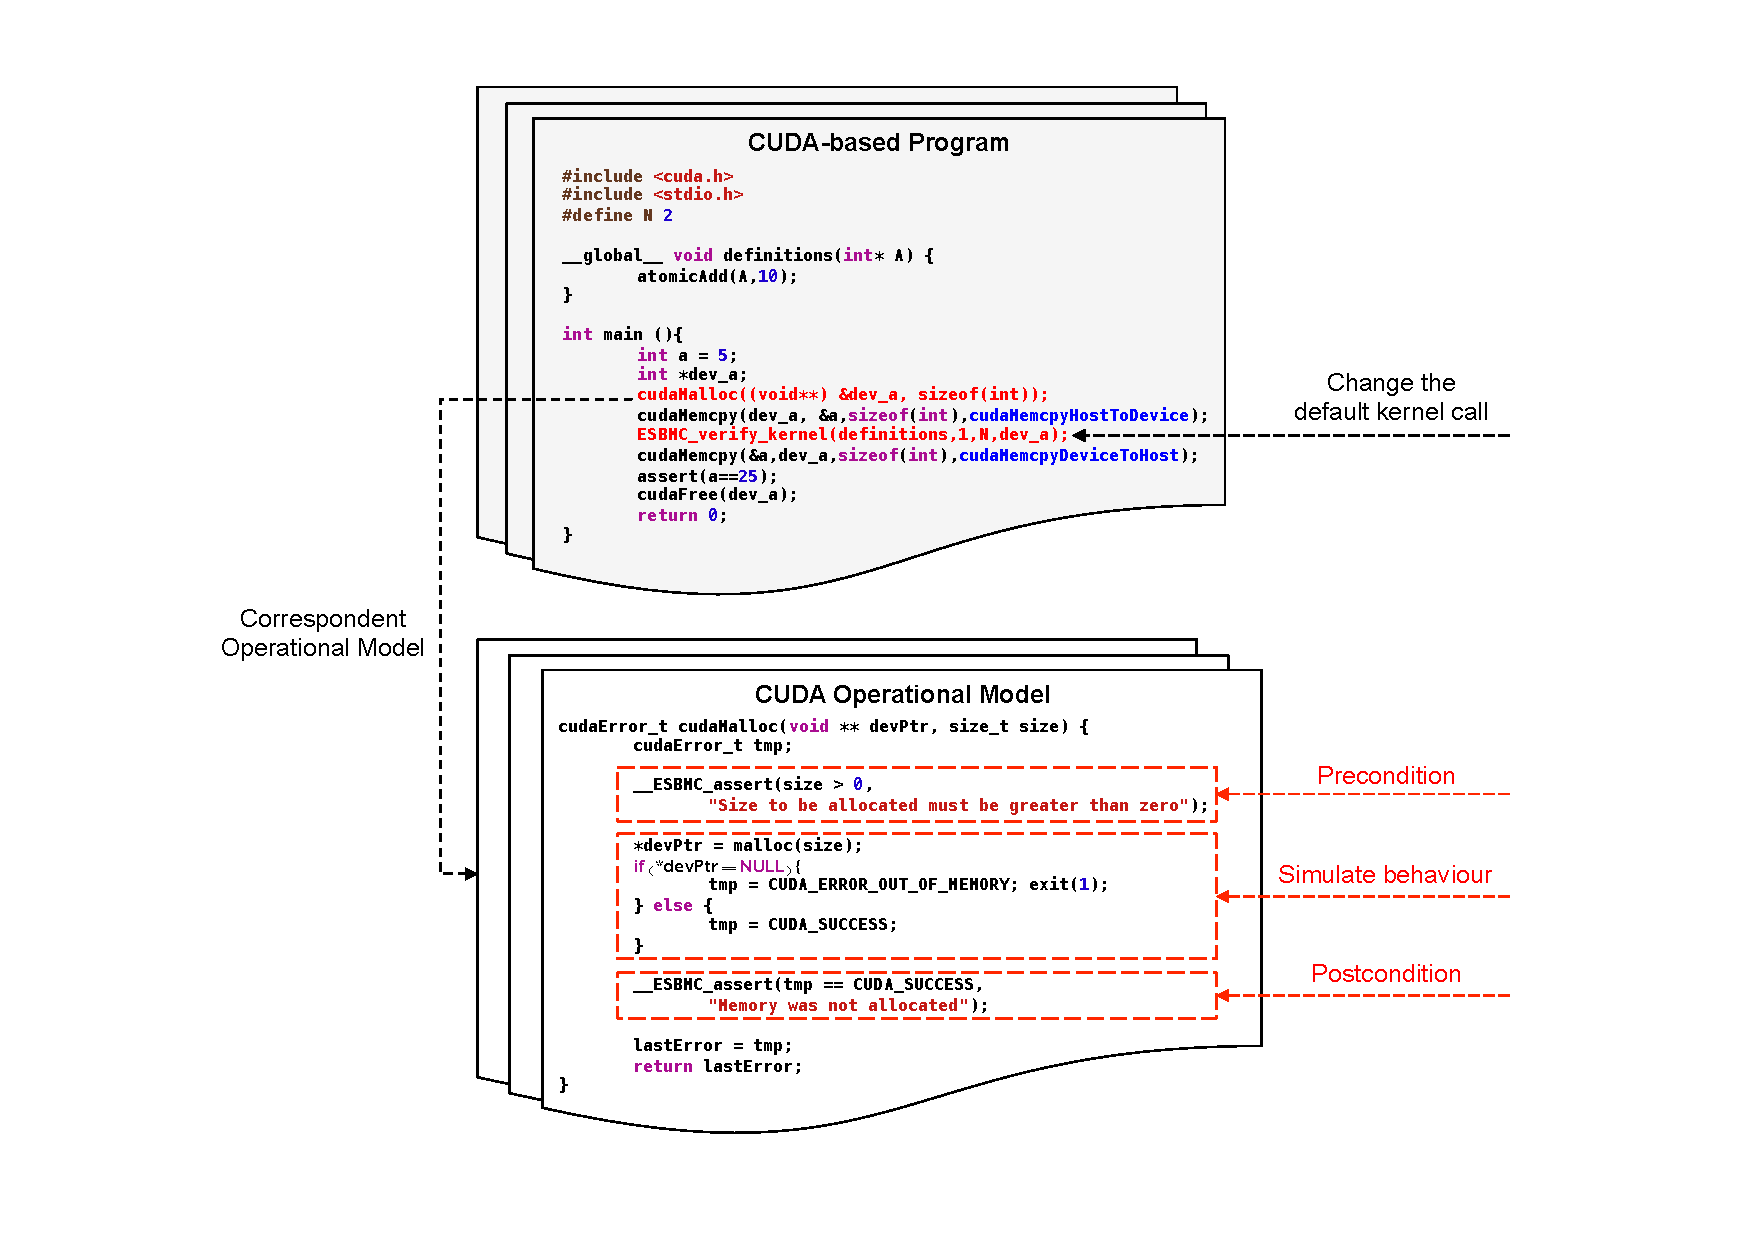
\includegraphics[width=4in]{figures/demo-om.pdf}
  			\caption{CUDA operational model scheme.}
  			\label{figure:demo-om}
		\end{figure}
		
		\begin{enumerate}
			\item As shown in Fig.~\ref{figure:demo-om}, operational models add assertions to the verification process, in order to check for specific properties;
			\item Verification model adopts the CPU parallel processing based on the POSIX Threading Library; \\
		\end{enumerate}

	\item Two-threads Analysis;
		
	Fig.~\ref{figure:demo-two} demonstrates the thread representation, which accesses the GPU shared memory and is based on NVIDIA Fermi GPU architecture. First of all, the numbered white boxes represent the shared memory positions to be accessed, ${t_{r}}^n$ are the thread-readers, and ${t_{w}}^n$ are the thread-writers, where $n$ is the index of each thread. %it is worth noticed that the threads are executed on a streaming multiprocessor. 
	In the first case of Fig.~\ref{figure:demo-two} (\textit{i.e.}, $S_{1}$), the threads, whose kernel is correctly implemented, do not present a data race condition, once they access different memory positions. In the second case of Fig.~\ref{figure:demo-two} (\textit{i.e.}, $S_{2}$), the threads execution of a kernel results in a data race condition, where several threads read or write in the same memory position, at the same lock-step. Finally, the third case of Fig.~\ref{figure:demo-two} is quite similar to the situation occurred in $S_{2}$, however, instead of using multiple threads to analyze data-race conditions, ESBMC-GPU ensures that such errors can be detected through the analysis of the behavior of two threads that are operating over the same memory location ({\it i.e.}, $S_3$).

		\begin{figure}[htb]
  			\centering
  			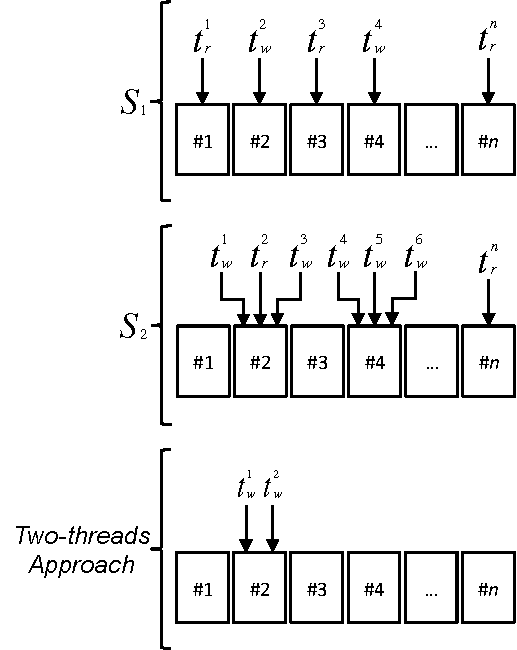
\includegraphics[width=2in]{figures/two-thread-approach.pdf}
  			\caption{Two-threads analysis.}
  			\label{figure:demo-two}
		\end{figure}
		
Note that the two-threads analysis affects mostly the data race verification, where program states must be analyzed with respect to their possible thread interleavings, which lead to an execution order of statements that results in error. In our benchmarks, we observed that the consideration of solely two threads attains substantial improvement in performance, whilst keeping true incorrect results at low rates.\\

%In our benchmarks, we observed a substantial performance improvement, considering only two threads, while keeping true incorrect results at low rates.\\
		
	\item State Hashing; 
	
	Our symbolic state hashing approach computes a summary for a particular state that has been explored, and then index the set of explored state to reduce the generation of redundant states. In particular, given any state computed during the symbolic execution of a specific CUDA kernel, we simply summarize it and efficiently look up whether it has been explored before, along a different computation path; if that happens during the ESBMC-GPU symbolic execution, then the current computation path does not need to be further explored in the reachability tree. So if we reach a state in ESBMC-GPU, where a context switch can be taken ({\it e.g.}, before a global variable or synchronization primitive), and all shared/local variables together with the program counters are similar to another explored node, then ESBMC-GPU just considers one identical node to be further explored, since reachability subtrees associated to identical nodes are also similar. \\

	\item Monotonic Partial Order Reduction;
	
		\begin{figure}[!]
			\begin{center}
    			\subfloat[Independent transitions\label{subfig-1:independent}]{%
      				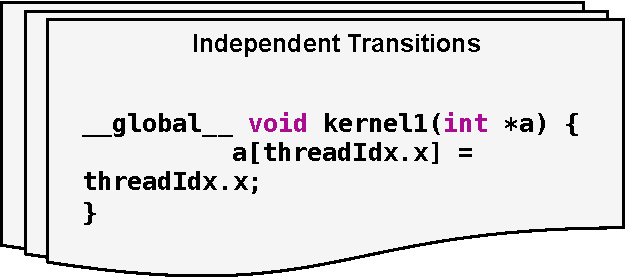
\includegraphics[width=0.45\textwidth]{figures/demo-mpor-a-code.pdf}
    			}
    			\hfill
    			\subfloat[Dependent transitions\label{subfig-2:dependent}]{%
      				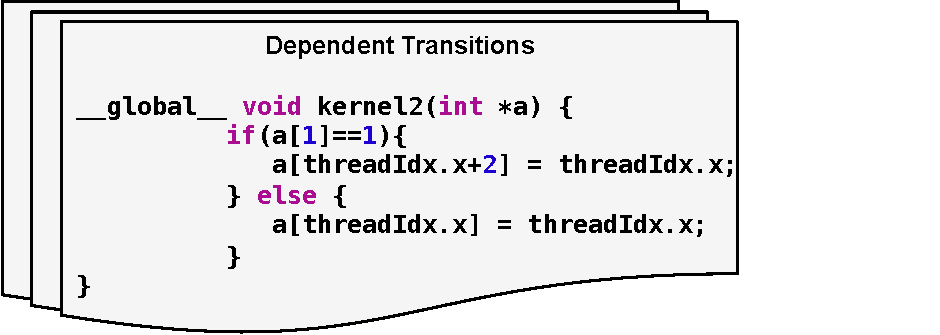
\includegraphics[width=0.45\textwidth]{figures/demo-mpor-b-code.pdf}
    			}
    			\caption{Code snippets of CUDA kernels.}
    			\label{figure:demo-mpor-codes}
		\end{center}
  		\end{figure}
		
	In order to understand MPOR algorithm, one can observe the code snippets shown in Fig.~\ref{figure:demo-mpor-codes}. In addition, Fig.~\ref{subfig-1:independent} shows the application of MPOR to a CUDA kernel, where the global variable $a$ is written in a position relative to the thread ID; in particular, this variable determines the program execution state. On the first interleaving, thread $t_{1}$ reaches $v_1$ resulting in $a=[0,0]$. Thread $t_{2}$ runs and reaches $v_2$ resulting in $a=[0,1]$. The MPOR algorithm then checks whether $v_2$ does not exist and whether transition $t_1 \rightarrow t_2$ is defined as independent. Both conditions do not hold, therefore transition $t_1 \rightarrow t_2$ is defined as dependent. ESBMC-GPU thus performs all possible interleavings, and the next execution starts with thread $t_2$ from $v_0$, which changes the array's content to $a=[0,1]$. Thread $t_1$ runs and reaches $v_4$, which is similar to $v_2$. MPOR algorithm then checks whether thread $t_1$ has reached a redundant state. As thread $t_1$ has only reached $v_1$, then the algorithm concludes that the transition $t_2 \rightarrow t_1$ is independent, disregarding it (represented in Fig.~\ref{subfig-1:independent} by dotted lines).

		\begin{figure}[!]
			\begin{center}
    			\subfloat[Independent transitions\label{subfig-1:independent}]{%
      				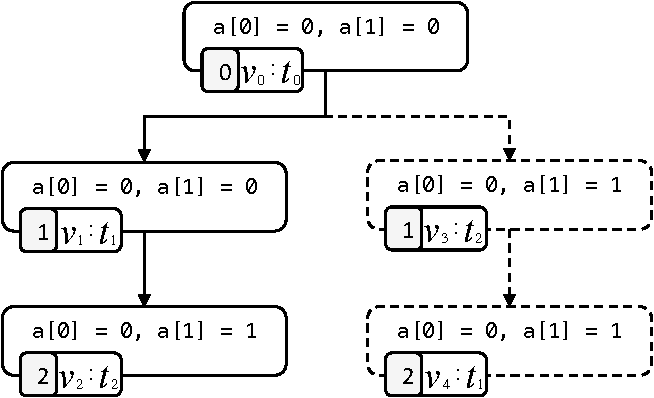
\includegraphics[width=0.45\textwidth]{figures/demo-mpor-a.pdf}
    			}
    			\hfill
    			\subfloat[Dependent transitions\label{subfig-2:dependent}]{%
      				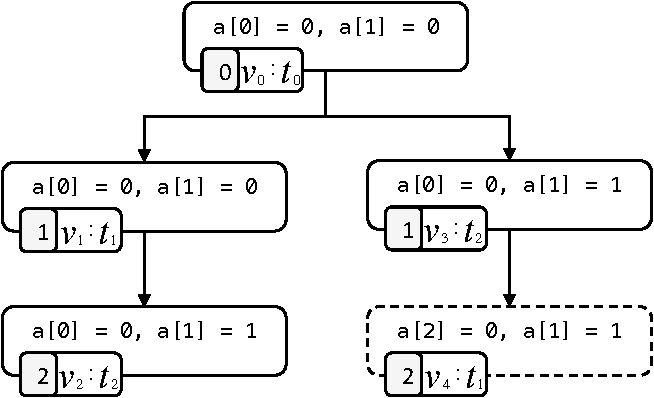
\includegraphics[width=0.45\textwidth]{figures/demo-mpor-b.pdf}
    			}
    			\caption{MPOR applied to a kernel with independent and dependent transitions.}
    			\label{figure:demo-mpor}
		\end{center}
  		\end{figure}
		
Fig.~\ref{subfig-2:dependent} shows another example in which the thread execution results in different states. On the first interleaving, the thread execution $t_1$ reaches $v_1$ and the thread execution $t_2$ reaches $v_2$. Since the content of $a[1]$ is different in both reachability tree (RT) nodes, the condition does not hold. On the second interleaving, thread $t_2$ modifies the array $a$ to $a=[0,1]$ and thread $t_1$ accidentally writes to $a[2]$. MPOR algorithm then checks whether $v_4$ exists in the RT. Since the condition does not hold, transition $t_2 \rightarrow t_1$ is then defined as dependent. In this particular case, both interleavings are considered and those two thread execution orders result in an array out-of-bounds violation since the array $a$ is of length $2$ (\textit{e.g.}, $v_4$ in dotted lines).\\

      \end{itemize}
  \end{itemize}
  \item ESBMC-GPU Demonstration (60\%)
\\

%\textcolor{red}{Felipe: There is too much repetition here w.r.t. section 4 Usage Aspects. Can you please focus your description based on a running example from the Microsoft suite? then you can show the code and how we use ESBMC-GPU to verify that program.}
  	%\begin{figure}[htb]
  	%	\centering
  	%	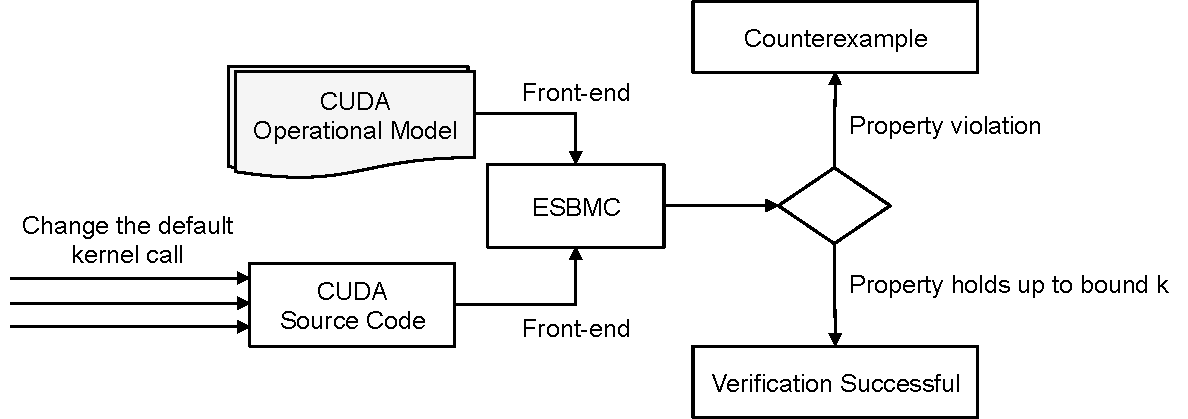
\includegraphics[width=4in]{figures/verification-flow.pdf}
  	%	\caption{ESBMC-GPU's verification flow.}
  	%	\label{figure:verification-flow}
	%\end{figure}

%\begin{figure} [htb]
%\centering
%\begin{minipage}{\textwidth}
%\begin{lstlisting}
%#include <call_kernel.h>
%#include <stdio.h>
%#include <stdlib.h>
%#include <stdio.h>
%#include <cuda.h>
%#include <cuda_runtime_api.h>
%#include <assert.h>
%__global__ void Asum(int *a, int *b, int *c){
%	*c = *a + *b;
%}
%int main(void){
%	int a, b, c;
%	int *dev_a, *dev_b, *dev_c;
%	int size = sizeof(int);
%	cudaMalloc((void**)&dev_a, size);
%	cudaMalloc((void**)&dev_b, size);
%	cudaMalloc((void**)&dev_c, size);
%	a = 2;
%	b = 7;
%	c = 8;	
%	cudaMemcpy(dev_a, &a, size, cudaMemcpyHostToDevice);
%	cudaMemcpy(dev_b, &b, size, cudaMemcpyHostToDevice);
%	// Asum<<<1,2>>>(dev_a, dev_b, dev_c);
%	ESBMC_verify_kernel(Asum, 1, 2, dev_a, dev_b, dev_c);
%	cudaMemcpy(&c, dev_c, size, cudaMemcpyDeviceToHost);
%	assert(c != a + b);	
%	cudaFree(dev_a);
%	cudaFree(dev_b);
%	cudaFree(dev_c);
%	return 0;
%}
%\end{lstlisting}
%\end{minipage}
%\caption{Illustrative CUDA code example.}
%\label{fig:illustrative}
%\end{figure}

\begin{figure} [htb]
\centering
\begin{minipage}{\textwidth}
\begin{lstlisting}
#include <call_kernel.h>
#include <stdio.h>
#include <stdlib.h>
#include <stdio.h>
#include <cuda.h>
#include <cuda_runtime_api.h>
#include <assert.h>

#define BLOCKS 1
#define THREADS 2

__global__ void kernel(int *A) {
	A[threadIdx.x + 1] = threadIdx.x;
}

int main(){
	int *a;
	int *dev_a;
	int size = THREADS*sizeof(int);
	a = (int*)malloc(size);
	cudaMalloc((void**)&dev_a, size);
	for (int i = 0; i < THREADS; i++)
		a[i] = 0;
	cudaMemcpy(dev_a, a, size, cudaMemcpyHostToDevice);
	// kernel<<<BLOCKS,THREADS>>>(dev_a);
	ESBMC_verify_kernel(kernel, BLOCKS, THREADS, dev_a);
	for (int i = 0; i < THREADS; i++)
		assert(a[i]==i);	
	cudaFree(dev_a);
	return 0;
}
\end{lstlisting}
\end{minipage}
\caption{Illustrative CUDA code example.}
\label{fig:illustrative-example}
\end{figure}

In this part, we will demonstrate the ESBMC-GPU usage, based on the CUDA program shown in Fig.~\ref{fig:illustrative-example}. First of all, the user must replace the default kernel call (line $25$) to an intrinsic function of ESBMC-GPU (line $26$), as explained in Sec.~\ref{subsec:usage}. Then, the modified CUDA program can be passed to the command-line version of ESBMC-GPU as follows:

\begin{center}
%\vspace{1 mm}
\noindent \texttt{esbmc-gpu} \emph{\tt <file>.cu} {\tt --unwind <$k$>}  {\tt --context-switch <$c$>}

\noindent {\tt --state-hashing} {\tt -I <path-to-CUDA-OM>},
%\vspace{1 mm}
\end{center}

%As one may see in Fig.~\ref{fig:illustrative-example}, this CUDA-based program has 1 block and 2 threads, respectively. Furthermore, its kernel (lines $8$ to $10$) stores in the variable $c$ the result of the sum of $a$ and $b$, which are passed as input arguments. However, there is a mistake in the assertion (line $26$), as $a + b$ must be equal to $c$, which is correctly detected by ESBMC-GPU detects an assert violation.

As one may see in Fig.~\ref{fig:illustrative-example}, this CUDA-based program has 1 block and 2 threads, and a kernel (lines $12$ to $14$), which assigns thread's index values to an array passed as an input argument. Indeed, its goal is to instantiate array positions according to the thread index. However, there is a mistake in the array index, as the value $1$ is accidentally added to the thread index (line $13$). As shown in the main function, array positions are assigned with value $0$ (line $23$), and after the kernel call (line $26$), it is expected that $a[0] == 0$ and $a[1] == 1$.

In this example, ESBMC-GPU detects an array out-of-bounds violation. Indeed, this CUDA-based program retrieves a memory region that has not been previously allocated, thus, when {\tt threadIdx.x = 1}, the program tries to access the position $a[2]$. Importantly, the {\tt cudaMalloc()} function operational model has a precondition that checks if the memory size to be allocated is greater than zero. In addition, an assertion checks if the result matches to the expected postcondition (line $28$). Therefore, the verification of this program through ESBMC-GPU produces $34$ successful and $6$ failed interleavings. For instance, one possible failed interleaving is represented by the threads executions $t_0 : a[1] = 0$; $t_1 : a[2] = 1$, where $a[2] = 1$ represents an incorrect access to the array index $a$.

It is worth noticing that ESBMC-GPU and GKLEE are able to detect this array out-of-bounds violation, but GPUVerify and PUG fail, as they report a true incorrect result (missed bug). Furthermore, ESBMC-GPU has the following additional command-line options: \\

%\texttt{--no-assertions}: to ignore assertions; \\
%\texttt{--no-bounds-check}: to skip array bounds check; \\
%\texttt{--no-div-by-zero-check}: to skip division by zero check; \\
%\texttt{--no-pointer-check}: to skip pointer check; \\
\texttt{--memory-leak-check}: to enable memory leak check; \\
\texttt{--overflow-check}: to enable arithmetic over- and underflow check; \\
%\texttt{--deadlock-check}: to enable global and local deadlock check with mutex; \\
\texttt{--data-races-check}: to enable data races check; \\
%\texttt{--lock-order-check}: to enable for lock acquisition ordering check; \\
%\texttt{--atomicity-check}: to enable atomicity check at visible assignments; \\
%\texttt{--memlimit}: to configure memory limit, of form ``100MB'' or ``2GB''; \\
%\texttt{--timeout}: to configure time limit, integer followed by \{s, m, or h\}; \\
%\texttt{--force-malloc-success}: to consider that there is always enough memory available in the device; \\
\texttt{-DGPU\_threads=<$number$>}: to define the total number of threads by kernel. \\

The tool, operational model, and all experiments results are available for downloading at: \texttt{http://esbmc-gpu.org/}.\\

Video demonstration at \texttt{https://www.youtube.com/watch?v=Q7pOAr6zY3c}.
\end{enumerate}

\end{document}

